% !Mode:: "TeX:UTF-8"
%% 请使用 XeLaTeX 编译本文.
% \documentclass{WHUBachelor}% 选项 forprint: 交付打印时添加, 避免彩色链接字迹打印偏淡. 即使用下一行:
 \documentclass[forprint]{WHUBachelor}
\usepackage{amsmath, amsfonts, amssymb} % math equations, symbols
\usepackage[english]{babel}
\usepackage{color}      % color content
\usepackage{graphicx}   % import figures
\usepackage{url}        % hyperlinks
\usepackage{bm}         % bold type for equations
\usepackage{multirow}
\usepackage{booktabs}
\usepackage{epstopdf}
\usepackage{epsfig}
\usepackage{algorithm}
\usepackage{algorithmic}
\usepackage{esvect}
\usepackage{listings}
\usepackage[framed,numbered,autolinebreaks,useliterate]{mcode}
\usepackage{subfig}
\usepackage{float}
\begin{document}
%%%%%%% 下面的内容, 据实填空.


\StudentNumber{2016011560} % 填写自己的学号

\title{\\Foundation of Finite Elements Method\\Assignment FEM model}

\author{易泽吉}                            % 作者名字

\Cmajor{工程力学}                  % 专业中文名

\Cschoolname{航天航空学院}          % 学院名

\date{二〇一八年三月}                    % 日期, 要注意和英文日期一致!!


%-----------------------------------------------------------------------------
\pdfbookmark[0]{封面}{title}         % 封面页加到 pdf 书签
\maketitle
\frontmatter
\pagenumbering{Roman}              % 正文之前的页码用大写罗马字母编号.
%-----------------------------------------------------------------------------

%==========================把目录加入到书签==============================%%%%%%
\pdfbookmark[0]{目录}{toc}
\mainmatter %% 以下是正文
%%%%%%%%%%%%%%%%%%%%%%%%%%%--------main matter-------%%%%%%%%%%%%%%%%%%%%%%%%%%%%%%%%%%%%
\section{Euler-Bernoulli Beam单元}
\subsection{单元构造}
每个梁单元有两个节点首先确定梁单元的位移向量与载荷向量。规定沿梁的轴线方向为x方向,单元的位移向量与载荷向量可以表示为:
\begin{equation} 
d^{e}=\left(\begin{array}{llllllllllll}{u_{x 1}} & {u_{y 1}} & {u_{z 1}} & {u_{x 1}} & {u_{y 1}} & {u_{z 1}} & {u_{x 2}} & {u_{y 2}} & {u_{z 2}} & {\theta_{x 2}} & {\theta_{y 2}} & {\theta_{y 3}}\end{array}\right)^{T}
 \end{equation}
\begin {equation} 
f^{e}=\left(\begin{array}{cccccccccccc}{F_{x 1}} & {F_{y 1}} & {F_{z 1}} & {M_{x 1}} & {M_{y 1}} & {M_{z 1}} & {F_{x 2}} & {F_{y 2}} & {F_{z 2}} & {M_{x 2}} & {M_{y 3}}\end{array}\right)^{T}
 \end {equation}
其中$u$表示位移,$\theta$表示转角,$f$表示剪力,$M$表示弯矩,下标中1,2分别表示两端节点。\par
对于梁单元有四个独立的模态,第一个为轴向拉伸,与杆单元相同,第二个为沿轴扭转,第三四个分别为垂直于轴线的两个方向的弯曲,单元的刚度矩阵如下,矩阵中各元素的值不需要高斯积分,可直接导出。
\begin{equation}
K^e=\left(\begin{array}{cccccccccccc}
   \frac{EA}{l} & 0 & 0 & 0 & 0 & 0 & -\frac{EA}{l} & 0 & 0 & 0 & 0 & 0\\
 & \frac{12EI_z}{l^3} & 0 & 0 & 0 & \frac{6EI_z}{l^2} & 0 & -\frac{12EI_z}{l^3} & 0 & 0 & 0 & \frac{6EI_z}{l^2} \\
 &  & \frac{12EI_y}{l^3} & 0 & -\frac{6EI_z}{l^2} & 0 & 0 & 0 & -\frac{12EI_y}{l^3} & 0 & -\frac{6EI_z}{l^2} & 0 \\
 &  &  & \frac{GJ_z}{I} & 0 & 0 & 0 & 0 & 0 & - \frac{GJ_z}{I} & 0 & 0\\
 &  &  &  & \frac{4EI_y}{l} & 0 & 0 & 0 & \frac{6EI_y}{l} & 0 & \frac{2EI_y}{l} & 0\\
 &  &  &  &  & \frac{4EI_z}{l} & 0 & -\frac{6EI_z}{l} & 0 & 0 & 0 & \frac{2EI_z}{l}\\
 &  \multicolumn{3}{c}{\raisebox{1.3ex}[0pt]{Symmetry}}  &  &  &\frac{EA}{l} & 0 & 0 & 0 & 0 & 0\\
 &  &  &  &  &  &  & \frac{12EI_z}{l^3} & 0 & 0 & 0 & -\frac{6EI_z}{l^2}\\
 &  &  &  &  &  &  &  & \frac{12EI_y}{l^3} & 0 & \frac{6EI_y}{l^2} & 0\\
 &  &  &  &  &  &  &  &  & \frac{GJ_z}{I} & 0 & 0\\
 &  &  &  &  &  &  &  &  &  & \frac{4EI_y}{l} & 0\\
 &  &  &  &  &  &  &  &  &  &  &\frac{4EI_z}{l}\\
\end{array}\right)
\end{equation}
在写出单元刚度阵以及位移向量之后,我们就得到了单元的控制方程:
\begin{equation} 
K^{e} d^{e}=f^{e}
 \end{equation}
这样就可以准备将单元刚度阵组装到总体刚度阵,当然在此之前需要将单元刚度阵做坐标变换,这源自于在全局的坐标系,真实的单元方程是:
\begin{equation} 
K^{e} R d^{e}= R f^{e}
 \end{equation}
因此有
\begin{equation} 
K^{global} = R^T K^{element} R
 \end{equation}
其中R为12*12的矩阵,其中有四个分块,每个分块都为方向余弦阵
\begin{equation} 
R = 
\begin{bmatrix}
A & & & \\
& A & & \\
& & A & \\
& & & A 
\end{bmatrix}
\end{equation}
其中A=
\begin{equation} 
\hat{A}=\left[\begin{array}{lll}{a_{x} a'_{x}} & {a_{x} a'_{y}} & {a_{x} a'_{z}} \\ {a_{y} a'_{x}} & {a_{y} a'_{y}} & {a_{y} a'_{z}} \\ {a_{z} a'_{x}} & {a_{z} a'_{y}} & {a_{z} a'_{z}}\end{array}\right]
 \end{equation}
将如此经过正交变换的单元刚度阵组装到总刚度阵即可
\subsection{梁单元的输入规定}
梁单元的在单元类型中编号为4,需要输入的材料性质包括基本的杨氏模量 E,泊松比$\mu$,另外本工程项目中使用的是空心矩形截面梁,为保证对称性,即保证不移轴,上下壁面的厚度需要相同,左右壁面的厚度需要相同,因此依次输入的参数是:矩形的长和宽(a,b),上下壁面的厚度,左右壁面的厚度,以及一组单位向量(n1,n2,n3)来表征局部坐标系的y轴在全局坐标系中的方向。考虑到桥梁中的梁单元都存在于xz平面,该向量可以被置为(0,1,0)
\subsection{Patch Test}
首先对于梁进行不规则的划分,如下图所示:

梁的总长度为1m,共划分为4个单元,5个节点,分别在$x=0,0.2,0.3,0.5,1$处。
\begin{figure}[H]
\centering
    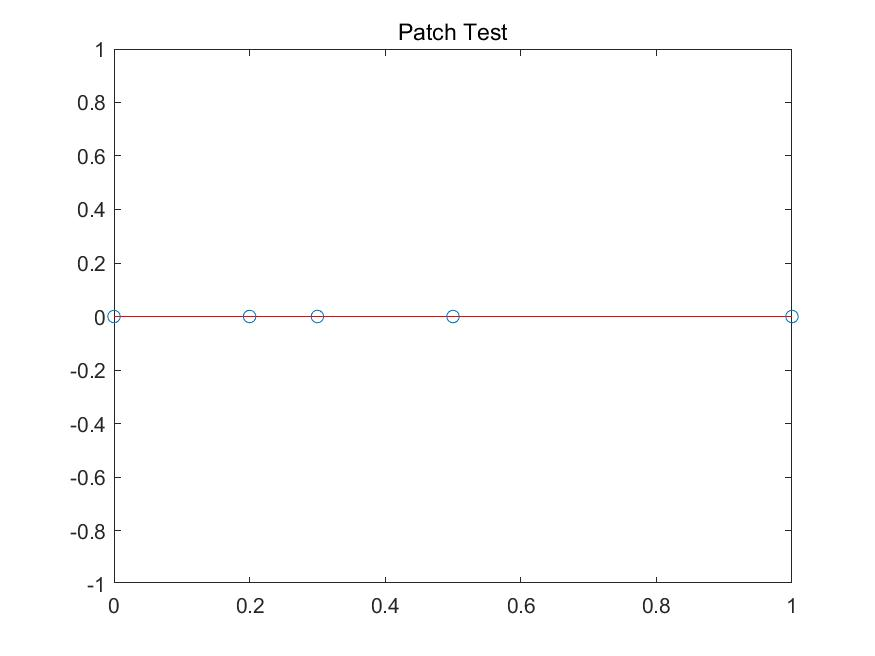
\includegraphics[width=.7\textwidth]{patch_test_beam.jpg}
  \caption{Patch Test}
\end{figure}
由于梁有四个互相独立解耦的模态,对其分别约束测试。\par
首先验证y方向挠度,即z方向弯曲,如下构造精确解。本质边界条件为两端简支,自然边界条件为两边施加等大反向弯矩,梁处于纯弯曲状态且弯矩相等,位移的精确解为:
\begin{equation} 
w= x^{2}- x, \theta=2 x-1
 \end{equation}
分片试验结果如下,
\begin{table}[H]
  \centering
  \caption{DISPLACEMENT-WZ}
    \begin{tabular}{lcccccc}
\hline
NODE & X-D&Y-D &Z-D &$\theta_X$-D &$\theta_Y$-D&$\theta_Z$-D \\
\hline
1 & 0.000e+00 & 0.000e+00 & 0.000e+00 & 0.000e+00 & 0.000e+00 & -1.000e+01 \\
2 & 0.000e+00 & -1.600e+01 & 0.000e+00 & 0.000e+00 & 0.000e+00 & -6.000e+00 \\
3 & 0.000e+00 & -2.100e+01 & 0.000e+00 & 0.000e+00 & 0.000e+00 & -1.000e+01 \\
4 & 0.000e+00 & -2.500e+01 & 0.000e+00 & 0.000e+00 & 0.000e+00 & 1.237e-15 \\
5 & 0.000e+00 & 0.000e+00 & 0.000e+00 & 0.000e+00 & 0.000e+00 & 1.000e+01 \\
\hline
 \end{tabular}%
\end{table}
之后验证z方向挠度,y方向弯曲,边界条件及载荷相同,位移的精确解也相同,节点和分片方式相同,结果如下
\begin{equation} 
w= x^{2}- x, \theta=2 x-1
 \end{equation}
分片试验结果如下,
\begin{table}[H]
  \centering
  \caption{DISPLACEMENT-WZ}
    \begin{tabular}{lcccccc}
\hline
NODE & X-D&Y-D &Z-D &$\theta_X$-D &$\theta_Y$-D&$\theta_Z$-D \\
\hline
1 & 0.000e+00 & 0.000e+00 & 0.000e+00 & 0.000e+00  & -1.000e+01 & 0.000e+00\\
2 & 0.000e+00 &0.000e+00 &  -1.600e+01 & 0.000e+00  & -6.000e+00& 0.000e+00 \\
3 & 0.000e+00 & 0.000e+00 & -2.100e+01 & 0.000e+00 & -1.000e+01 & 0.000e+00 \\
4 & 0.000e+00 & 0.000e+00 & -2.500e+01 & 0.000e+00  & 9.877e-16 & 0.000e+00\\
5 & 0.000e+00 & 0.000e+00 & 0.000e+00 & 0.000e+00  & 1.000e+01 & 0.000e+00\\
\hline
 \end{tabular}%
\end{table}
x方向位移与杆单元的patch test相同,$\theta_x$方向应满足线性收敛率,结果如下
\begin{table}[H]
  \centering
  \caption{DISPLACEMENT-THETAX}
    \begin{tabular}{lcccccc}
\hline
NODE & X-D&Y-D &Z-D &$\theta_X$-D &$\theta_Y$-D&$\theta_Z$-D \\
\hline
1 & 0.000e+00 & 0.000e+00 & 0.000e+00 & 0.000e+00  & 0.000e+00 & 0.000e+00\\
2 & 0.000e+00 &0.000e+00 &0.000e+00 & 2.000e+00  & 0.000e+00& 0.000e+00 \\
3 & 0.000e+00 & 0.000e+00 & 0.000e+00 & 3.000e+00 & 0.000e+00 & 0.000e+00 \\
4 & 0.000e+00 & 0.000e+00 & 0.000e+00 & 5.000e+00  &0.000e+00 & 0.000e+00\\
5 & 0.000e+00 & 0.000e+00 & 0.000e+00 & 1.000e+01  & 0.000e+00 & 0.000e+00\\
\hline
 \end{tabular}%
\end{table}
\subsection{收敛性分析}
选取悬臂梁,调整重力大小,即均布载荷大小,构造出精确解:
梁单元可以有效重构三次位移场,因此,带有均布载荷的悬臂梁可以较好的反应误差。
\begin{equation} 
w=0.01 x^{4}
 \end{equation}
误差范数采用位移范数,可以表示为
\begin{equation} 
\|e\|^2=\int A\left(u-u^{h}\right)^{2} d x
 \end{equation}
计算收敛率时网格划分如下:
\begin{figure}[H]
\centering
  \subfloat[1element]{%
    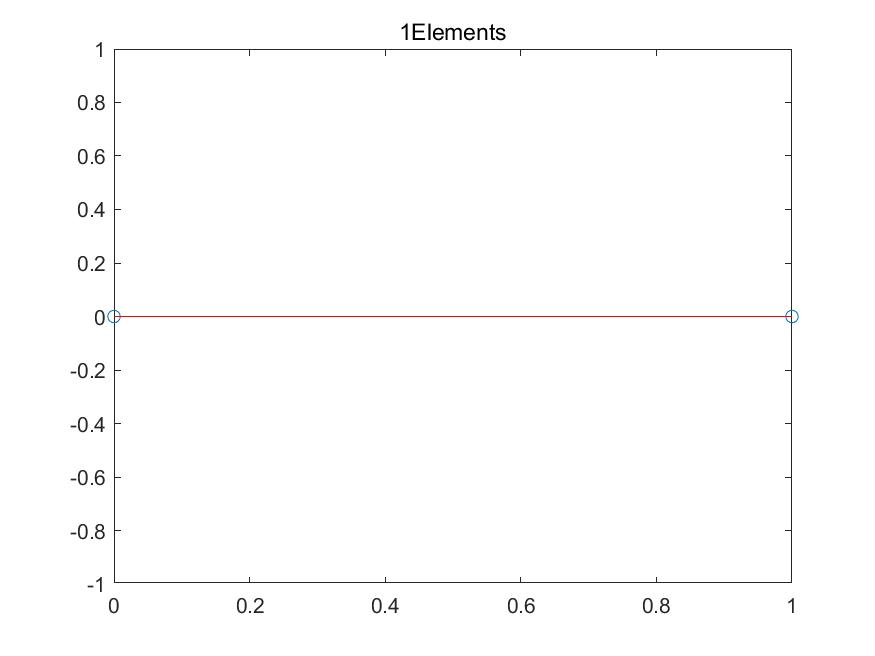
\includegraphics[width=.3\textwidth]{conv_rate0.jpg}}\hfill
  \subfloat[2elements]{%
    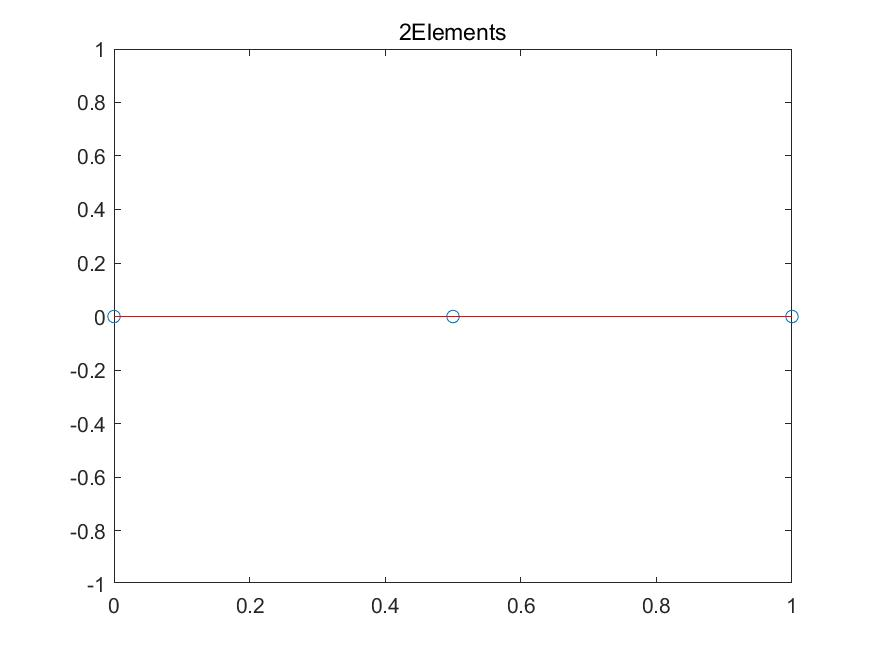
\includegraphics[width=.3\textwidth]{conv_rate1.jpg}}\hfill
\subfloat[3elements]{%
    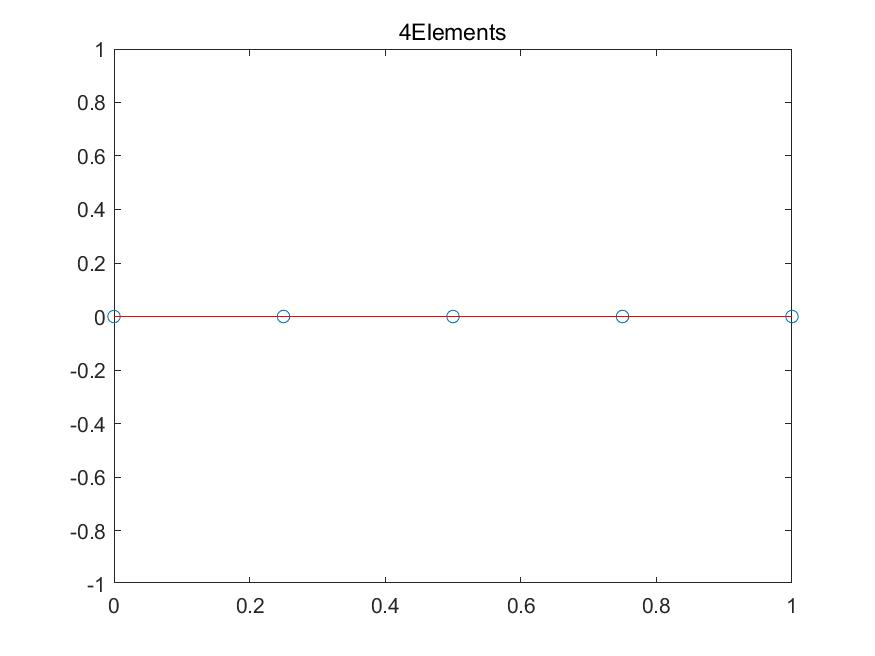
\includegraphics[width=.3\textwidth]{conv_rate2.jpg}}\\

  \subfloat[4elements]{%
    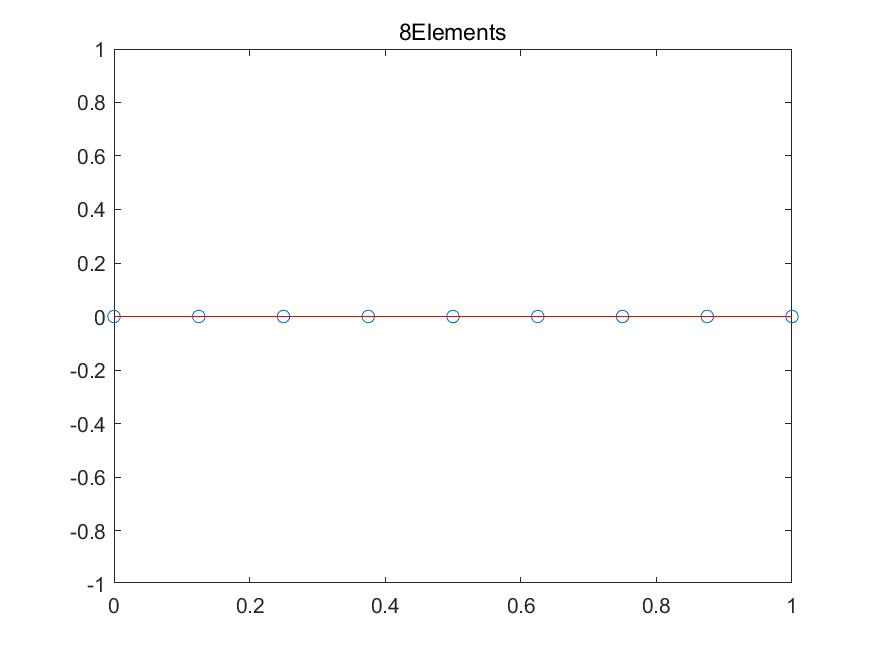
\includegraphics[width=.3\textwidth]{conv_rate3.jpg}}\hfill
 \subfloat[5elements]{%
    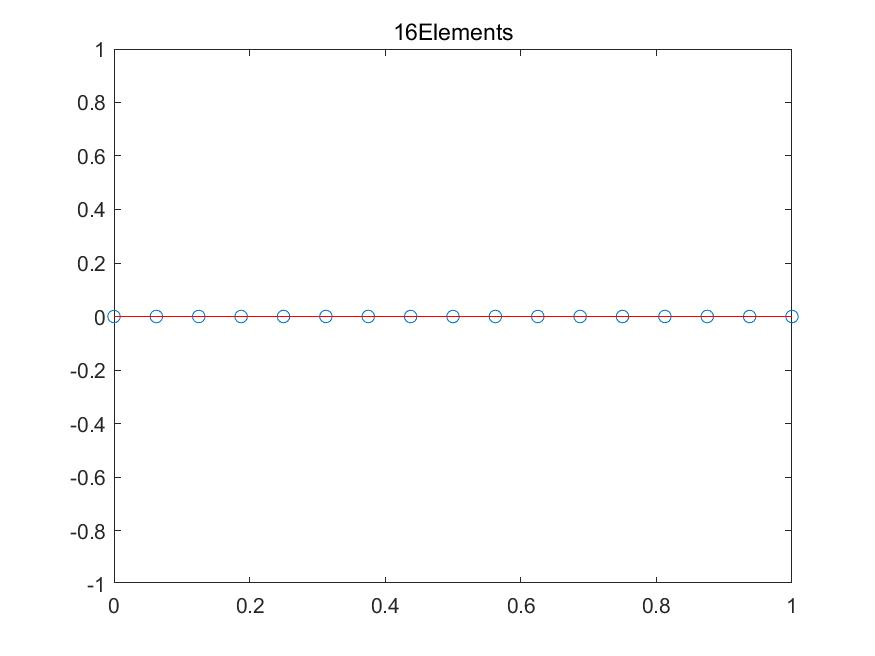
\includegraphics[width=.3\textwidth]{conv_rate4.jpg}}\hfill
\subfloat[6elements]{%
    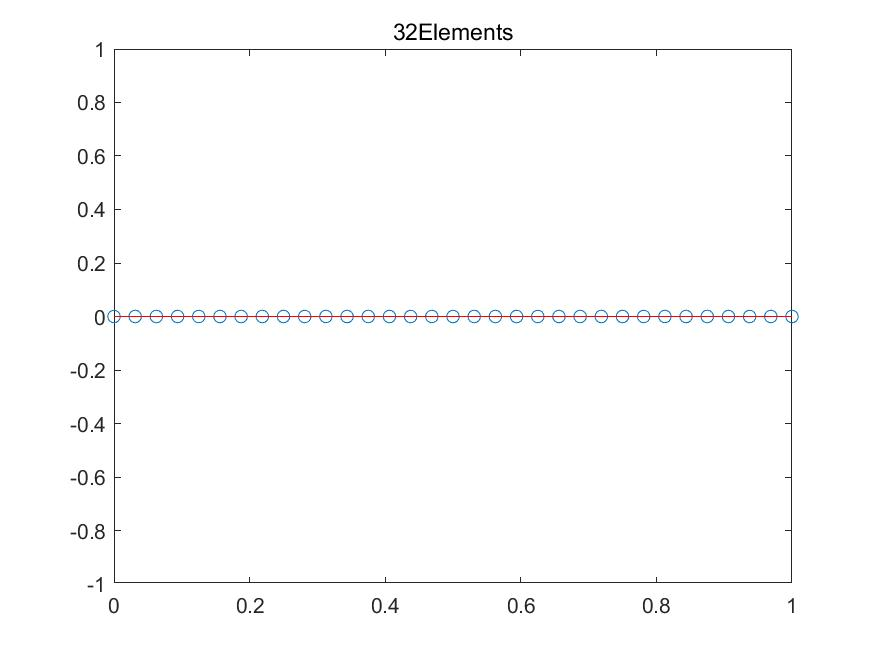
\includegraphics[width=.3\textwidth]{conv_rate5.jpg}}\\
  \caption{Convergence Mesh}\label{fig:2}
\end{figure}
最终收敛率结果如图所示:
\begin{figure}[H]
\centering
    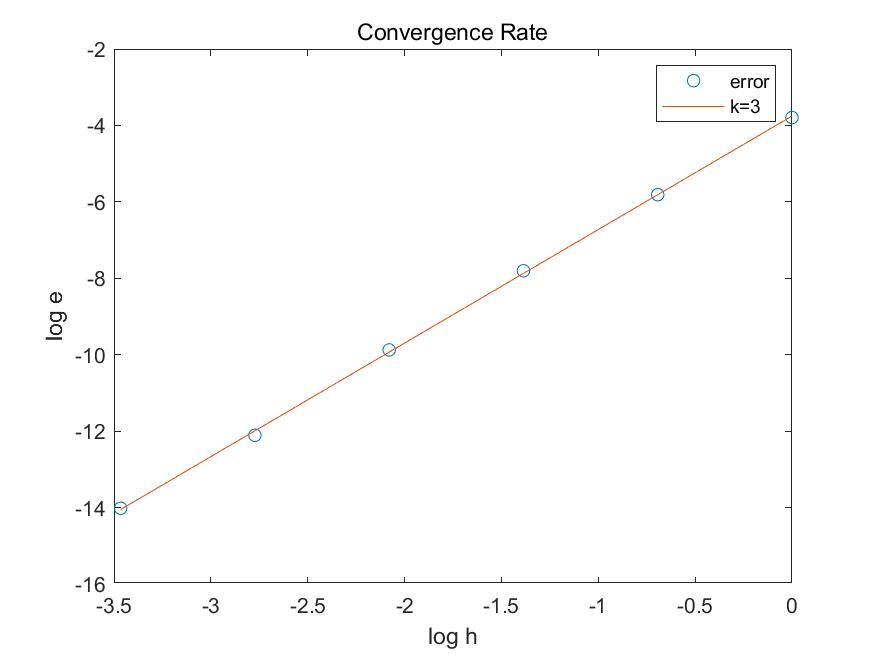
\includegraphics[width=.7\textwidth]{beam_conv_rate.jpg}
  \caption{Convergence Rate}
\end{figure}
\section{Timoshenko Beam}
\subsection{Timoshenko Beam的基本假设}
Euler–Bernoulli梁适用于薄梁,忽略横向剪切变形,横向剪切应力由平衡方程确定,不适用于有效长度较短的梁或组合梁。Timoshenko梁仍然假设与梁轴线垂直的横截面在变形后保持平面(假设为刚性横截面平面),但放松了一些约束,即放弃了直法线假设,采用剪应变沿截面均匀分布的假设,在一定程度上解决了欧拉伯努利梁的问题。
\subsection{Timoshenko Beam 的控制方程}
从变分原理出发有,系统的势能泛函为
\begin{equation} 
\Pi_{P}=\int_{0}^{l} \frac{1}{2} E I\left(\frac{\mathrm{d} \theta}{\mathrm{d} x}\right)^{2} \mathrm{d} x+\int_{0}^{l} \frac{1}{2} \frac{G A}{k} \gamma^{2} \mathrm{d} x-\int_{0}^{l} q w \mathrm{d} x
 \end{equation}
其中,
\begin{equation} 
\varepsilon_{x}=-z \frac{\mathrm{d} \theta}{\mathrm{d} x} \quad \gamma=\frac{\mathrm{d} w}{\mathrm{d} x}-\theta \quad \kappa=-\frac{\mathrm{d} \theta}{\mathrm{d} x}
 \end{equation}
按照有限元格式离散之后可以写成
\begin{equation} 
\begin{aligned} \Pi_{P} &=\int_{0}^{l} \frac{1}{2} E I\left(\frac{\mathrm{d} \theta}{\mathrm{d} x}\right)^{2} \mathrm{d} x+\int_{0}^{l} \frac{1}{2} \frac{G A}{k} \gamma^{2} \mathrm{d} x-\int_{0}^{l} q w \mathrm{d} x \\ &=\sum_{e}\left[\int_{\Omega^{e}} \frac{1}{2} E I\left(\frac{\mathrm{d} \theta}{\mathrm{d} x}\right)^{2} \mathrm{d} x+\int_{\Omega^{e}} \frac{1}{2} \frac{G A}{k} \gamma^{2} \mathrm{d} x-\int_{\Omega^{e}} q w \mathrm{d} x\right] \\ &=\frac{1}{2} \sum_{e}\left(\boldsymbol{d}^{e}\right)^{\mathrm{T}}\left[\left(\boldsymbol{K}_{b}^{e}+\boldsymbol{K}_{s}^{e}\right) \boldsymbol{d}^{e}-f^{e}\right] \end{aligned}
 \end{equation}
其中
\begin{equation} 
\begin{aligned} \boldsymbol{K}_{b}^{e} &=\int_{\Omega^{e}} E I \boldsymbol{B}_{b}^{e \mathrm{T}} \boldsymbol{B}_{b}^{e} \mathrm{d} x \\ \boldsymbol{K}_{s}^{e} &=\int_{\Omega^{e}} \frac{G A}{k} \boldsymbol{B}_{s}^{e \mathrm{T}} \boldsymbol{B}_{s}^{e} \mathrm{d} x \\ \boldsymbol{f}^{e} &=\int_{\Omega^{e}} \boldsymbol{N}^{e \mathrm{T}}\left[\begin{array}{c}{q} \\ {0}\end{array}\right] \mathrm{d} x \end{aligned}
 \end{equation}
根据最小势能原理有
\begin{equation} 
\delta \Pi_{P}=0
 \end{equation}
从而
\begin{equation} 
\begin{array}{l}{E I_{z} \frac{d \kappa_{z}}{d x}+\frac{G A}{k} \gamma_{x y}+\overline{M}_{z k} \delta\left(x-x_{k}\right)=0} \\ {\frac{G A}{k} \frac{d \gamma_{x y}}{d x}+\overline{q}+\overline{N}_{y j} \delta\left(x-x_{j}\right)=0}\end{array}
 \end{equation}
即
\begin{equation} 
\delta \boldsymbol{d}^{\mathrm{T}}\left(\sum_{e} \boldsymbol{L}^{e \mathrm{T}}\left(\boldsymbol{K}_{b}^{e}+\boldsymbol{K}_{s}^{e}\right) \boldsymbol{L}^{e} \boldsymbol{d}-\sum_{e} \boldsymbol{L}^{e \mathrm{T}} \boldsymbol{f}^{e}\right)=0 \quad \forall \boldsymbol{d}_{F}
 \end{equation}
\subsection{有限元离散与插值函数}
我们选取的插值方式为位移转角的一致插值,即考虑两种模式,一种为欧拉伯努利梁,只有弯曲位移,没有剪切位移,另一种为简单修正,只有剪切位移,没有弯曲位移:
\begin{equation} 
\begin{aligned} a &=a_{b}+a_{s} \\ a_{i} &=\left(u_{i}, v_{i}, w_{i}, \varphi_{i}, \theta_{y i}, \theta_{z i}\right)^{T} \\ a_{b} &=\left(a_{b 1}, a_{b 2}\right)^{T} \\ a_{s} &=\left(a_{s 1}, a_{s 2}\right)^{T} \\ a_{b i} &=\left(u_{i}, v_{b i}, w_{b i}, \varphi_{i}, \theta_{y i}, \theta_{z i}\right)^{T} \\ a_{s i} &=\left(0, v_{s i}, w_{s i}, 0,0,0\right)^{T} \end{aligned}
 \end{equation}
对于欧拉伯努利梁的模式,弯曲所产生的变形与转角有如下关系:
\begin{equation} 
\begin{aligned} \frac{d v_{b i}}{d x} &=\theta_{z i} \\ \frac{d w_{b i}}{d x} &=-\theta_{y i} \end{aligned}
 \end{equation}
下面我们选取y,z中的任意方向,进行插值和推导,对于欧拉伯努利梁部分,采用Hermite插值
\begin{equation} 
v_{b}=N_{1} v_{b 1}+N_{2} \theta_{1}+N_{3} v_{b 2}+N_{4} \theta_{4}
 \end{equation}
对于剪切部分,采用两点线性插值
\begin{equation} 
v_{s}=N_{5} v_{s 1}+N_{6} v_{s 2}
 \end{equation}
其中$\xi$为母单元坐标值
\begin{equation} 
\begin{array}{ll}{N_{1}=1-3 \xi^{2}+2 \xi^{3}} & {N_{2}=\left(\xi-2 \xi^{2}+\xi^{3}\right)}l \\ {N_{3}=3 \xi^{2}-2 \xi^{3}} & {N_{4}=\left(\xi^{3}-\xi^{2}\right) l} \\ {N_{5}=1-\xi} & {N_{6}=\xi}\end{array}
 \end{equation}
将插值函数代入有
\begin{equation} 
\boldsymbol{B}_{b}^{e}=\left[\begin{array}{ccc} \frac{\mathrm{d} N_{1}}{\mathrm{d} x} & \ldots & \frac{\mathrm{d} N_{n}}{\mathrm{d} x}\end{array}\right]
 \end{equation}
由于单元内部平衡方程$Q=\frac{d M}{d x}$,欧拉伯努利梁部分与剪力部分有如下关系
\begin{equation} 
\left(\begin{array}{c}{v_{b 2}-v_{b 1}} \\ {v_{s 2}-v_{s 1}}\end{array}\right)=\left(\begin{array}{cc}{\frac{1}{1+b_{z}}} & {\frac{l b_{z}}{2\left(1+b_{z}\right)}} \\ {\frac{b_{z}}{1+b_{z}}} & {-\frac{l b_{z}}{2\left(1+b_{z}\right)}}\end{array}\right)\left(\begin{array}{c}{v_{2}-v_{1}} \\ {\theta_{z 1}+\theta_{z 2}}\end{array}\right)
 \end{equation}
其中,$b_{z} :=\frac{12 E I_{z} k}{G A l^{2}}$,对于矩形截面梁的近似有$k=\frac{6}{5}$。整理之后可以得到,
$\boldsymbol{K} \boldsymbol{d}=\boldsymbol{F}$
其中
\begin{equation} 
\boldsymbol{K}=\frac{E I_{z}}{\left(1+b_{z}\right) l^{3}}\left(\begin{array}{cccc}{12} & {-12} & {6 l} & {6 l} \\ { } & {12} & {-6 l} & {-6 l} \\ { } & { } & {\left(4+b_{z}\right) l^{2}} & {\left(2-b_{z}\right) l^{2}} \\ {[\text {symmetry}]} & & & {\left(4+b_{z}\right) l^{2}} \end{array}\right)
 \end{equation}
考虑所有分量的问题,同时加入扭转以及拉压方向的问题
\begin{equation} 
\boldsymbol{a}=\boldsymbol{a}_{b}+\boldsymbol{a}_{s}
 \end{equation}
有如下刚度阵
\begin{equation}
\setlength{\arraycolsep}{1pt}
\left(\begin{array}{cccccccccccc}
  \frac{EA}{l} & 0 & 0 & 0 & 0 & 0 & -\frac{EA}{l} & 0 & 0 & 0 & 0 & 0\\
 & \frac{12EI_z}{(1+b_z)l^3} & 0 & 0 & 0 & \frac{(1+b_z)6EI_z}{l^2} & 0 & -\frac{12EI_z}{l^3} & 0 & 0 & 0 & \frac{6EI_z}{(2-b_z)l^2} \\
 &  & \frac{12EI_y}{(1+b_y)l^3} & 0 & -\frac{6EI_z}{(1+b_y)l^2} & 0 & 0 & 0 & -\frac{12EI_y}{(1+b_y)l^3} & 0 & -\frac{6EI_z}{(1+b_y)l^2} & 0 \\
 &  &  & \frac{GJ_z}{I} & 0 & 0 & 0 & 0 & 0 & - \frac{GJ_z}{I} & 0 & 0\\
 &  &  &  & \frac{(4+b_y)EI_y}{(1+b_y)l} & 0 & 0 & 0 & \frac{6EI_y}{(1+b_y)l} & 0 & \frac{(2-b_y)EI_y}{(1+b_y)l} & 0\\
 &  &  &  &  & \frac{(4+b_z)EI_z}{(1+b_z)l} & 0 & -\frac{6EI_z}{(1+b_z)l} & 0 & 0 & 0 & \frac{(2-b_z)EI_z}{(1+b_z)l}\\
 &  \multicolumn{3}{c}{\raisebox{1.3ex}[0pt]{Symmetry}}  &  &  &\frac{EA}{l} & 0 & 0 & 0 & 0 & 0\\
 &  &  &  &  &  &  & \frac{12EI_z}{(1+b_z)l^3} & 0 & 0 & 0 & -\frac{6EI_z}{(1+b_z)l^2}\\
 &  &  &  &  &  &  &  & \frac{12EI_y}{(1+b_y)l^3} & 0 & \frac{6EI_y}{(1+b_y)l^2} & 0\\
 &  &  &  &  &  &  &  &  & \frac{GJ_z}{I} & 0 & 0\\
 &  &  &  &  &  &  &  &  &  & \frac{(4-b_y)EI_y}{(1+b_y)l} & 0\\
 &  &  &  &  &  &  &  &  &  &  &\frac{(4-b_y)EI_z}{(1+b_z)l}\\
\end{array}\right)
\end{equation}
同时单元应力的具体计算公式如下:
\begin{equation} 
\begin{aligned} \sigma_{x x} &=E \varepsilon_{x x}=\frac{E\left(u_{2}-u_{1}\right)}{l} \\ \sigma_{x y} &=\frac{G}{k} \gamma_{x y} \\ &=\frac{G}{k l} \frac{b_{z}}{1+b_{z}}\left(\left(v_{2}-v_{1}\right)-\frac{1}{2}\left(\theta_{z 1}+\theta_{z 2}\right) l\right) \\ \sigma_{x z} &=\frac{G}{k} \gamma_{x z} \\ &=\frac{G}{k l} \frac{b_{y}}{1+b_{y}}\left(\left(w_{2}-w_{1}\right)+\frac{1}{2}\left(\theta_{y 1}+\theta_{y 2}\right) l\right) \end{aligned}
 \end{equation}
\subsection{程序实现}
在Stappp程序中新增了Timoshenko单元,在基类Material的基础上派生了CTimoshenkoMaterial类,Timoshenko梁的裁量性质与Beam相同,同时在程序实现时需要注意坐标的转换,我们得出的刚度阵是在单元坐标系中得出的,我们需要将其转换到全局坐标系组装。与Beam单元类似,有
\begin{equation} 
K^{e} R d^{e}= R f^{e}
 \end{equation}
因此有
\begin{equation} 
K^{global} = R^T K^{element} R
 \end{equation}
其中R为12*12的矩阵,其中有四个分块,每个分块都为方向余弦阵
\begin{equation} 
R = 
\begin{bmatrix}
A & & & \\
& A & & \\
& & A & \\
& & & A 
\end{bmatrix}
\end{equation}
其中A=
\begin{equation} 
\hat{A}=\left[\begin{array}{lll}{a_{x} a'_{x}} & {a_{x} a'_{y}} & {a_{x} a'_{z}} \\ {a_{y} a'_{x}} & {a_{y} a'_{y}} & {a_{y} a'_{z}} \\ {a_{z} a'_{x}} & {a_{z} a'_{y}} & {a_{z} a'_{z}}\end{array}\right]
 \end{equation}
将如此经过正交变换的单元刚度阵组装到总刚度阵即可
\subsection{Patch Test}
对于Timoshenko单元,我们考虑其常应变模态为常曲率与常剪应变状态,对于位移与转角有:
\begin{equation} 
\begin{aligned} v &=\frac{1}{2} a x^{2}+c x+d \\ \theta_{z} &=a x+b \end{aligned}
 \end{equation}
注意到此处转角并非单纯位移的积分,因为剪力项对于位移有线性贡献儿对于转角无贡献。这一状态实际上对应于一端集中剪力载荷与弯矩载荷共同作用的悬臂梁。此处选取两种精确解进行patch test的测试。首先为常弯曲状态,即悬臂梁一端施加弯矩。具有如下精确解
\begin{equation} 
w=0.5x^{2}, \theta= x
 \end{equation}
分片试验结果如下:
\begin{figure}[H]
\centering
  \subfloat[1element]{%
    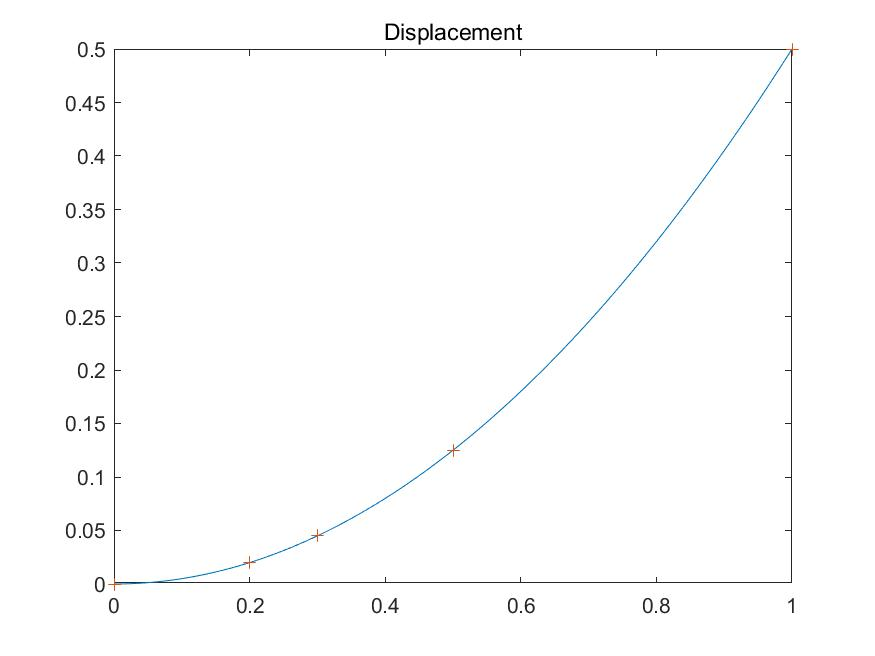
\includegraphics[width=.5\textwidth]{Timo_patch_dis.jpg}}\hfill
  \subfloat[2elements]{%
    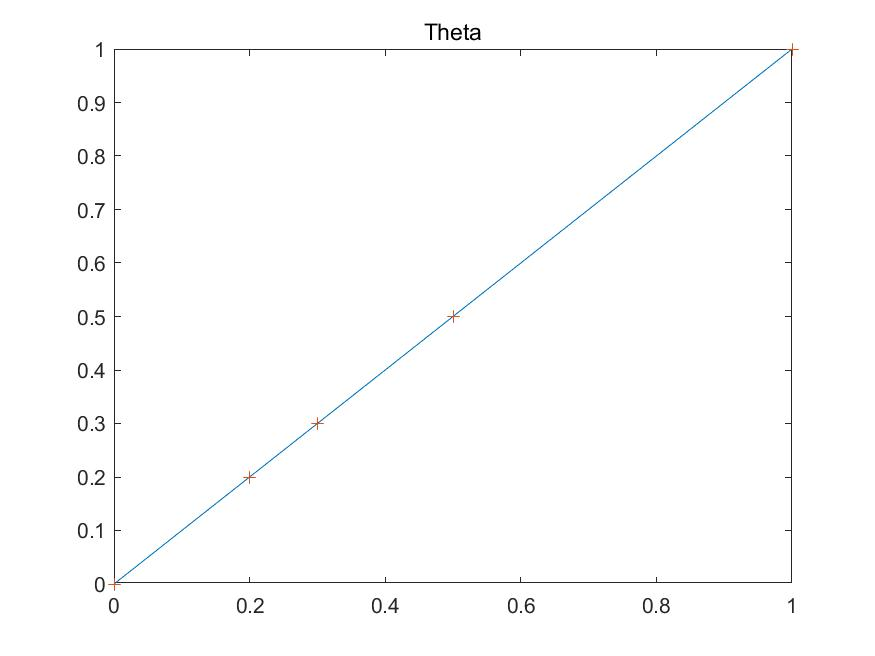
\includegraphics[width=.5\textwidth]{Timo_patch_theta.jpg}}\hfill

  \caption{Timoshenko Beam Patch Test 1}\label{fig:2}
\end{figure}
其次对于纯剪应力状态,精确解为
\begin{equation} 
w=-x^3+3x^{2}+x, \theta= -3x^2+6x
 \end{equation}
分片试验结果如下:
\begin{figure}[H]
\centering
  \subfloat[1element]{%
    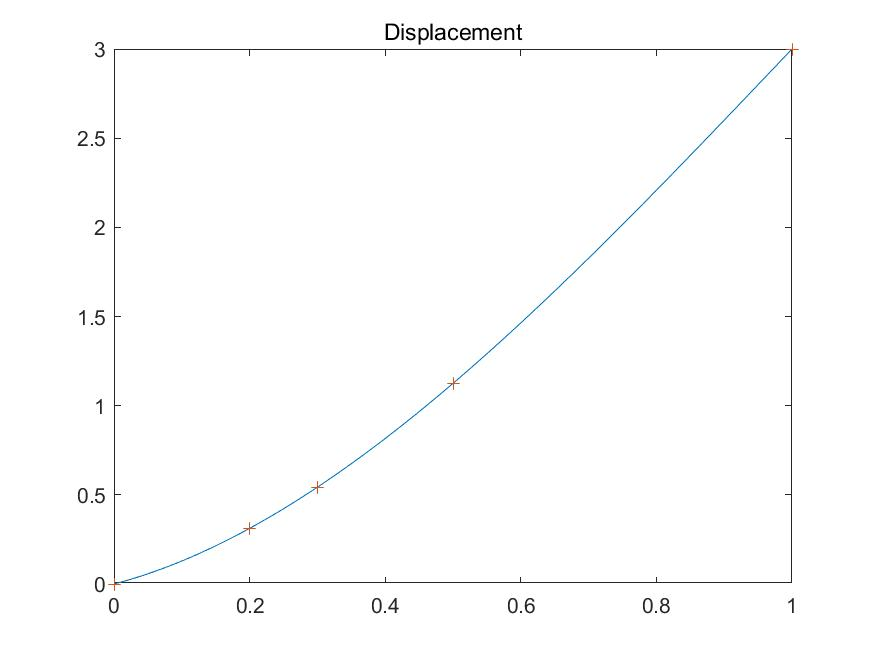
\includegraphics[width=.5\textwidth]{Timo_patch2_dis.jpg}}\hfill
  \subfloat[2elements]{%
    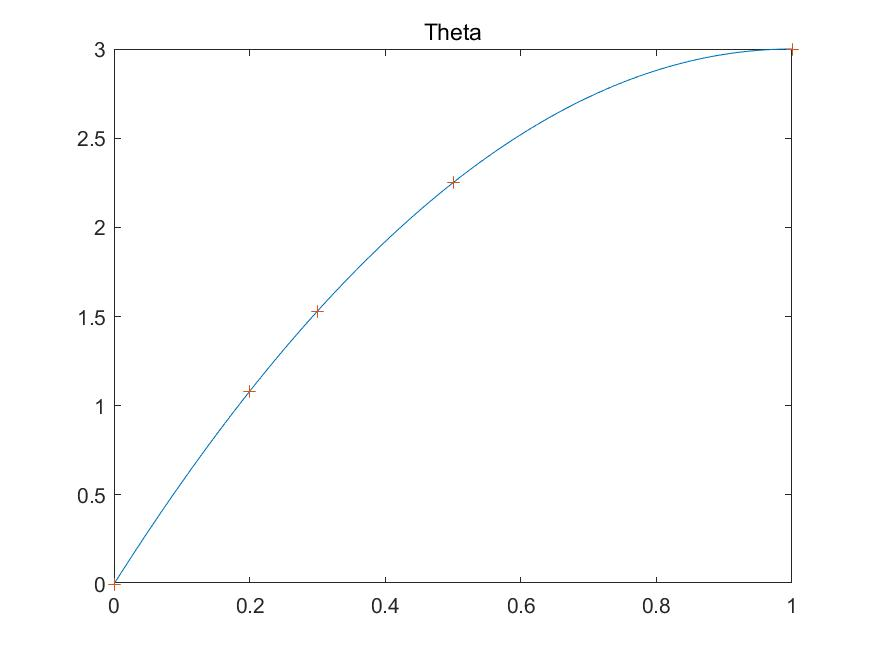
\includegraphics[width=.5\textwidth]{Timo_patch2_theta.jpg}}\hfill

  \caption{Timoshenko Beam Patch Test 2}\label{fig:2}
\end{figure}

\subsection{收敛率验证}
选取均布载荷,对于转角验证收敛率,精确解为三次函数,选取位移范数,收敛率如图
\begin{figure}[H]
\centering
    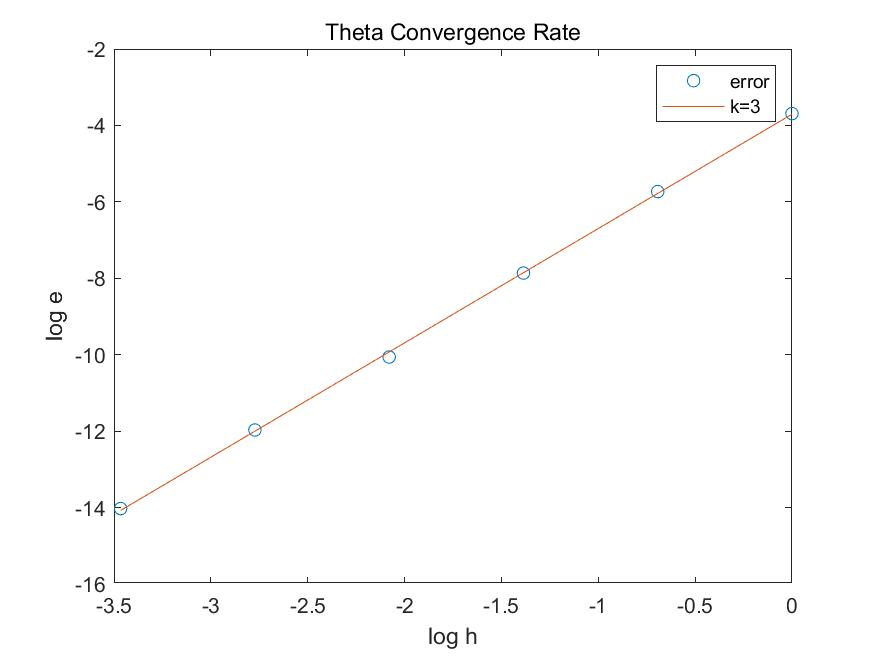
\includegraphics[width=.7\textwidth]{Timobeam_conv_rate.jpg}
  \caption{Convergence Rate}
\end{figure}
\section{稀疏矩阵求解器}
我们选取了MKL库中的稀疏矩阵求解器PARDISO,PARDISO的基本原理是根据稀疏特性优化的LDLT分解算法,基于共享内存,同时具有多线程的并行性,是一种Left-looking Right-looking 结合的算法。
\subsection{稀疏矩阵的存储方式}
CSR是最流行和通用的格式,可为高性能架构中的结构化和非结构化稀疏矩阵提供出色的压缩比。 具有CSR格式的向量运算在CPU上实现时显示出良好的性能改进,并且所有算法(如BLAS,LAPACK和CUSparse)均支持此格式。 它使用三个1维数组,一个用于保存非零值,第二个用于保存每行非零值的数量,第三个用于保存非零值的列索引。此格式的大小主要取决于矩阵中的非零值的数量。 CSR较好的反映了矩阵的稀疏特性,并且受每行非零值的分布的影响。
\begin {equation} 
A_{\operatorname{man}}=\left[ \begin{array}{ccccc}{0} & {4} & {0} & {7} & {0} \\ {2} & {0} & {3} & {0} & {6} \\ {0} & {5} & {0} & {0} & {0} \\ {0} & {0} & {0} & {0} & {2} \\ {1} & {0} & {0} & {6} & {0}\end{array}\right]
 \end {equation}

\begin{equation} 
Data=\left[ \begin{array}{ccccccccc}{4} & {7} & {2} & {3} & {6} & {5} & {2} & {1} & {6}\end{array}\right]
 \end{equation}
\begin{equation} 
Column-indices=\left[ \begin{array}{lllllllll}{1} & {3} & {0} & {2} & {4} & {1} & {4} & {0} & {3}\end{array}\right]
 \end{equation}
\begin{equation} 
P t r=\left[ \begin{array}{llllll}{0} & {2} & {5} & {6} & {7} & {9}\end{array}\right]
 \end{equation}
CSR占据的存储空间为
\begin{equation} 
CSR_{\text {storage}}=2 \times N Z V+m+1
 \end{equation}
\subsection{稀疏矩阵的具体实现}
在原有的STAP++的LDLT求解器中适配的是Skyline格式的矩阵,对于Pardiso求解器,适配上述的CSR格式的求解器。CSR格式需要矩阵每一行的长度来分配内存,但在组装过程结束前并不能完全清楚每一行的长度,因此这设计到可变长度的存储非零元素的索引值,因此我们考虑到使用c++的<vector>容器来进行存储。\par
在最终使用vector之前我们对比了其他c++标准STL容器。他们具有一些共同优点,如接口简单,排序速度快,使用方便,内存分配科学。但在这一问题中,vector的特点适配的较好。vector是典型的序列容器,唯一可以和标准C兼容的stl容器,任意元素的读取、修改具有常数时间复杂度,在序列尾部进行插入、删除是常数时间复杂度,但在序列的头部插入、删除的时间复杂度是O(n),可以在任何位置插入新元素,有随机访问功能,插入删除操作需要考虑。排序的时间复杂度为O(NlogN)。
在程序的编写过程中,首先扫描全部元素,标记所有非零元的位置,为CSR求解器预先分配内存之后对存储的索引值进行排序,去掉重复的索引值,之后分配矩阵元素值的存储空间。
\subsection{PARDISO的参数调节}
根据系统的环境可以调节系统的并行线程数,在16核的系统上性能得到了大幅度的提升。同时打开OOC模式开关,MKL带有IC/OOC模式的开关,IC指的是IN-CORE的存储,OOC指的是out-of-core的存储方式,通俗的说IC模式将原本全部存储在内存中的文件中超出允许使用的内存上限的部分存储在硬盘中,因此解决了内存溢出的问题。OOC可以通过将矩阵因子保存在磁盘上的文件中来解决非常大的问题,与IC相比,这减小了对于内存的需求。通过MKL-PARDISO-OOC-MAX-CORE-SIZE这一变量规定OOC模式PARDISO能够使用的最大内存量。同时在工作目录下配置pardiso-ooc.cfg配置文件。
我们在本地电脑上对于第二个算例进行了OOC的尝试,配置文件为:\\
ooc-max-core-size got from config file=200 \\
ooc-max-swap-size got from config file=0 \\
ooc-keep-file     got from config file=1 \\
显示成功读取相关配置文件
最终结果如下:
\begin{table}[htbp]
  \centering
  \caption{PARDISO STATISTICS}

    \begin{tabular}{lcl}
   \multicolumn{3}{l}{TIMES} \\
 \hline
Time spent in calculations of symmetric matrix portrait (fulladj)&:& 0.115191 s \\
Time spent in reordering of the initial matrix (reorder)         &:& 0.394719 s \\
Time spent in symbolic factorization (symbfct)                  & :& 0.589268 s \\
Time spent in data preparations for factorization (parlist)     & :& 0.013076 s \\
Time spent in copying matrix to internal data structure (A to LU)&:& 0.000000 s \\
      Factorization: Time for writing to files & :& 0.000000 \\
      Factorization: Time for reading from files&:& 0.000000 \\
Time spent in factorization step (numfct)       &                 : &76.839788 s\\
      Solution:      Time for reading from files&: &0.505685 \\
Time spent in direct solver at solve step (solve)&                : &0.623790 s \\
Time spent in allocation of internal data structures (malloc)&    : &3.694331 s \\
Time spent in additional calculations                        &    : &0.765964 s \\
Total time spent                                             &    : &83.036128 s \\
\hline
    \end{tabular}%
  \label{tab:addlabel}%
\end{table}%
\begin{table}[H]
  \centering
  \caption{OUT OF CORE STATISTICS}

    \begin{tabular}{lcl}
\multicolumn{3}{c}{ ----------- Out of core time (in percent) --------------} \\
\hline
\multicolumn{3}{l}{Factorization step(100):} \\
      write to files & : & 0 \\
      read from files&:& 0 \\ 
      factorization - write and read&:& 100 \\
\hline 
\multicolumn{3}{l}{Solution step (100):} \\
      read from files&:& 81 \\
      solve - writeread&:& 19 \\
Total time (100):& & \\
      read from files&:& 0 \\
      total - write and read&: &100 \\
----------- Out of core Mb -------------- \\
Factorization step:& &\\
      write to files &:&      0.000 Mb\\
      read from files&: &     0.000 Mb\\
Solution step: & & \\
      read from files&:&    414.116 Mb \\
Total size of data transferred:&  & \\
      write and read    & :  &  414.116 Mb\\
\hline
    \end{tabular}%

  \label{tab:addlabel}%

\end{table}%

同时OOC模式解决了第四个算例的内存溢出的问题,通过将大部分的存储内容放在硬盘中,用时间换空间,具备了解决大型问题的能力。例如:{\color{red}原本第四个算例我们的计算会发生内存溢出的问题,无法求解,现在通过OOC模式,将矩阵存储在硬盘中,完成了第四个算例的求解,可能是全班唯一具备求解第四个算例的能力的小组},但很遗憾的是,我们现在第四个算例的求解时间大约在30分钟左右,超出了求解时间,这可以在未来通过进一步的优化来解决,但OOC模式使得求解超大型的问题具备了理论可能,当然对于矩阵的结构等可能也需要进一步的优化,以减轻对存储容量的需求。\par
另外在求解过程中,我们也通过任务管理器对程序运行所占据的内存和CPU使用率进行了监控,在实验室的测试平台中,第四个算例中,程序8线程运行,CPU基本一直接近满负荷运行,内存最高峰达到50GB,磁盘的读写速度最高达到了500MB/s级别的速度,在本地测试的第二个算例中,内存高峰达到了400MB,在IC模式下为700MB,但程序运行时磁盘的读写速度大幅度上升,达到了50MB/s,整体运行时间增长了4倍左右。\par
如果运行环境的磁盘的读写速度有较大幅度的提升,如更换为SSD固态硬盘,可能对程序整体的运行时间有较好的增益,同时可以进一步分配更大的可使用内存量,当前考虑到系统的安全,我们只分配了大约45G的可使用内存空间。这在未来都是可以考虑优化的方面。
%\section{5.1}
%Point D,N,I:vicinity of point load.Point B,F,J,M:re-entrant conrners.
%\section{5.2}

%For NbN method $f_1 = 3q/8$,$f_2 = (q/4+2q/3)*5/2 = 55q/24$,$f_3 = (2q/3+11q/12)*3/2=57q/24$,$f_4 = (q+11q/12)/2 = 23q/24$.\par
%For EbE method  $f_1 = 3q/4$,$f_2 = 3q/4 + 4q/3 = 25q/12$,$f_3 = (11q/12+4q/3)=27q/12$,$f_4 = 11q/12$.\par
%Both the lumping method gurantee the resultant force is correct.The EbE method also satisfy the equivalence principle i.e. gurantee the resultant torque.
%\section{5.3}
%\begin{figure}[H]
%\centering
%  \subfloat[a]{%
%    \includegraphics[width=.3\textwidth]{a.png}}\hfill
%  \subfloat[b]{%
%    \includegraphics[width=.3\textwidth]{b.png}}\hfill
%\subfloat[c]{%
%    \includegraphics[width=.3\textwidth]{c.png}}\\
%
%  \subfloat[d]{%
%    \includegraphics[width=.3\textwidth]{d.png}}\hfill
% \subfloat[e]{%
%    \includegraphics[width=.3\textwidth]{e.png}}\hfill
%\subfloat[f]{%
%    \includegraphics[width=.3\textwidth]{f.png}}\\
%  \caption{Symmetry and asymmetry lines and Boudary condition}\label{fig:2}
%\end{figure}
%For problem a,the vertical and horizontal diameter is symmetry and the D BCs is along the lines.\\
%For problem b,both the 45degree direction is the antisymmetry line and the D BCs is vertical to the lines.\\
%For problem c,the horizontal line is antisymmetry line and the D BC is vertical.\\
%For problem d,the vertical and horizontal line is symmetry line and D BCs is along the line.\\
%For problem d,the vertical line alone the concentrated load is symmetry line and D BC is along the line.\\
%For problem e,the vertical line placed in the middle of the loads is antisymmetry line and D BCs is horizontal.
%\chapter{Appendix}
%I'm truly sorry that the images is rather ugly because I don't have sufficient PS skills(or other drawing applicant). Sincere thanks to TA for enduring that!
%\chapter{Abaqus Python Scripts}
%For the given Loads,considering the capacity of computer,I chose the following test cases.
%% Table generated by Excel2LaTeX from sheet 'Sheet1'
%\begin{table}[htbp]
%  \centering
%  \caption{Value of $\varphi$ $\theta$}
%    \begin{tabular}{|l|rrrrrrrrrrrr|}
%\hline
%    $\varphi$   & -90   & -75   & -60   & -45   & -30   & -15   & 0     & 15    & 30    & 45    & 60    & 75 \\
%    $\theta$ & 0     & 30    & 60    & 90    &       &       &       &       &       &       &       &  \\
%\hline
%    \end{tabular}%
%  \label{tab:addlabel}%
%\end{table}%/////
%The Result of the models is shown below. The whole model's internal energy met its minimum in the following cases.
%% Table generated by Excel2LaTeX from sheet 'Sheet1'

%The optimal values are
%\begin{equation}
%\begin{cases}
%\varphi = -30,E=40594& \theta = 0 \\
%\varphi = 30,E=29151& \theta = 30 \\
%\varphi = 30,E=11177& \theta = 60 \\
%\varphi = 0,E=3543& \theta = 90 \\
%\end{cases}
%\end{equation}
%The optimal internal energy cases's stress nephogram is given below.
%\begin{figure}[H]
%\centering
%  \subfloat[$\theta = 0 ,\phi = -30$]{%
%    \includegraphics[width=.5\textwidth]{T0P-30.png}}\hfill
%  \subfloat[$\theta = 30 ,\phi = 30$]{%
%    \includegraphics[width=.5\textwidth]{T30P30.png}}\\
%  \subfloat[$\theta = 60 ,\phi = 30$]{%
%    \includegraphics[width=.5\textwidth]{T60P30.png}}\hfill
% \subfloat[$\theta = 90 ,\phi = 0$]{%
%    \includegraphics[width=.5\textwidth]{T90P0.png}}\\
%  \caption{Stress nephogram}\label{fig:2}
%\end{figure}
%%%============================================================================================================%%%
%%%=== 参考文献 ========%%%

\cleardoublepage
\end{document}



